\documentclass[a4paper]{article}
\usepackage{amsmath}
\usepackage{graphicx}
\usepackage{hyperref}
\usepackage{bbm}

\title{Object Detection}
\author{SSW}

\begin{document}
\maketitle
\tableofcontents

\section{Model}
Model is the core
\subsection{Convolution}
\subsubsection{depth-wise convolution}
\subsubsection{group convolution}
\subsubsection{dilated convolution}
\subsubsection{deformable convolution}

\subsection{Normalization}

\subsection{Activation Function}


\begin{figure}[!h]
    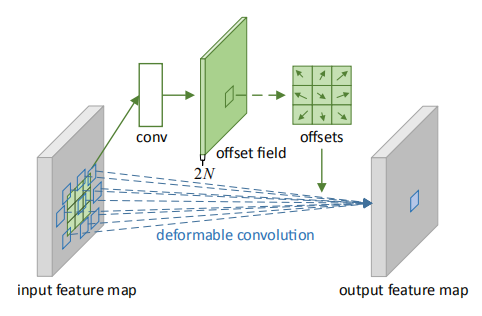
\includegraphics[width=\linewidth]{dcn.png}
    \caption{dcn}\label{fig:dcn}
\end{figure}

Refer to Figure~\ref{fig:dcn}, deformable convolution.
\[
    \text{cost} = -\mathbbm{1}_{\{c_i \ne \emptyset\}} \hat{p}_{\sigma(i)}(c_i) + \mathbbm{1}_{\{c_i \ne \emptyset\}}\mathcal{L}_{\text{box}}(b_i, \hat{b}_{\sigma(i)})
\]
\end{document}